\documentclass[25pt, a0paper, portrait, innermargin=4cm, colspace=2.5cm]{tikzposter}
\geometry{paperwidth=80cm}
% load packages
\usepackage[utf8]{inputenc}
\usepackage{mathpazo}
\usepackage[sfdefault,light]{roboto}
\usepackage[T1]{fontenc}
\usepackage{amsmath} 
\usepackage{blindtext}
\usepackage{comment}
\usepackage{enumerate}
\usepackage{xcolor}
\usepackage{boolexpr}
\usepackage{multicol}
\usetikzlibrary{arrows, decorations.markings}

% define default font
\renewcommand{\familydefault}{\sfdefault}

% define column separation
\setlength{\columnsep}{2cm}

% color definitions
\definecolor{tublue}{HTML}{3571A1}
\definecolor{tulightblue}{HTML}{589DD4}
\definecolor{tuorange}{HTML}{F6C07C}

% block style definitions
\defineblockstyle{myDefault}{titlewidthscale=1, bodywidthscale=1, titleleft, titleoffsetx=0pt, titleoffsety=0cm, bodyoffsetx=0cm, bodyoffsety=-1cm, bodyverticalshift=0pt, roundedcorners=0, linewidth=0.1cm, titleinnersep=.05cm, bodyinnersep=0cm}
{\begin{scope}[line width=\blocklinewidth, rounded corners=\blockroundedcorners]
    \ifBlockHasTitle
        %\draw[draw=none]
        %    (blockbody.south west) rectangle (blocktitle.north east);
        \draw[color=tuorange, solid, line width=2mm]
        (blocktitle.south west) -- (blocktitle.south east);
        %\draw[color=tublue, solid, line width=2mm]
        %([yshift=-2mm]blocktitle.south west) -- ([yshift=-2mm]blocktitle.south east);
    \else
        \draw[draw=none]
            (blockbody.south west) rectangle (blockbody.north east);
    \fi
\end{scope}}

% define title style
\definetitlestyle{myWave}{width=\paperwidth, roundedcorners=0, linewidth=0pt, innersep=1.5cm, titletotopverticalspace=0mm, titletoblockverticalspace=35mm, titlegraphictotitledistance=10pt, titletextscale=2}
{
    \coordinate (topleft) at (\titleposleft,\titlepostop);
    \coordinate (topright) at (\titleposright,\titlepostop);
    \coordinate (lefttoright) at (\titlewidth,0);
    \coordinate (head) at (0,\titlepostop-\titleposbottom);
    \coordinate (bottomright) at (\titleposright,0);
    %
    \draw[draw=none, left color=tublue, right color=tublue]%
        (topright) -- %
        (topleft) -- %
        ($(topleft) - (head)$) -- %
        ($(topright) - (head)$) -- cycle; %
    \draw[draw=none, left color=tuorange, right color=tuorange]%
        ($(topright) - (head)$ ) --  %
        ($(topleft) - (head)$) -- %
        ($(topleft) - (head)-(0,.5)$) -- %
        ($(topright) - (head)-(0,.5)$) -- cycle; %
    \draw[draw=none, left color=tulightblue, right color=tulightblue]%
        ($(topright) - (head)-(0,.5)$ ) --  %
        ($(topleft) - (head)-(0,.5)$) -- %
        ($(topleft) - (head)-(0,1.2)$) -- %
        ($(topright) - (head)-(0,1.2)$) -- cycle; %
    \draw[draw=none, left color=tublue, right color=tublue]%
        ($(topright) - (head)-(0,1.2)$ ) --  %
        ($(topleft) - (head)-(0,1.2)$) -- %
        ($(topleft) - (head)-(0,1.5)$) -- %
        ($(topright) - (head)-(0,1.5)$) -- cycle; %
    \draw[draw=none, left color=tublue, right color=tublue]%
        (bottomleft) --  %
        ($(bottomleft) + (\titlewidth, 0)$) -- %
        ($(bottomleft) + (\titlewidth, 8)$) -- %
        ($(bottomleft) + (0, 8)$) -- cycle; %
    \draw[draw=none, left color=tuorange, right color=tuorange]%
        ($(bottomleft) + (0, 8)$) -- %
        ($(bottomleft) + (\titlewidth, 8)$) -- %
        ($(bottomleft) + (\titlewidth, 8.5)$) -- %
        ($(bottomleft) + (0, 8.5)$) -- cycle; %
    \draw[draw=none, left color=tulightblue, right color=tulightblue]%
        ($(bottomleft) + (0, 8.5)$) -- %
        ($(bottomleft) + (\titlewidth, 8.5)$) -- %
        ($(bottomleft) + (\titlewidth, 9.2)$) -- %
        ($(bottomleft) + (0, 9.2)$) -- cycle; %
    \draw[draw=none, left color=tublue, right color=tulightblue]%
        ($(bottomleft) + (0, 9.2)$) -- %
        ($(bottomleft) + (\titlewidth, 9.2)$) -- %
        ($(bottomleft) + (\titlewidth, 9.5)$) -- %
        ($(bottomleft) + (0, 9.5)$) -- cycle; %
}

% define color palette
\definecolorpalette{sampleColorPalette} {
  \definecolor{colorOne}{named}{tublue}
  \definecolor{colorTwo}{named}{tuorange}
  \definecolor{colorThree}{named}{tulightblue}
}

% set color styles
\definecolorstyle{sampleColorStyle} {
  \definecolor{colorOne}{named}{blue}
  \definecolor{colorTwo}{named}{yellow}
  \definecolor{colorThree}{named}{orange}
  }{
  % Background Colors
  \colorlet{backgroundcolor}{white}
  \colorlet{framecolor}{white}
  % Title Colors
  \colorlet{titlefgcolor}{white}
  \colorlet{titlebgcolor}{tublue}
  % Block Colors
  \colorlet{blocktitlebgcolor}{white}
  \colorlet{blocktitlefgcolor}{tublue}
  \colorlet{blockbodybgcolor}{white}
  \colorlet{blockbodyfgcolor}{black}
  % Innerblock Colors
  \colorlet{innerblocktitlebgcolor}{white}
  \colorlet{innerblocktitlefgcolor}{black}
  \colorlet{innerblockbodybgcolor}{black}
  \colorlet{innerblockbodyfgcolor}{black}
  % Note colors
  \colorlet{notefgcolor}{black}
  \colorlet{notebgcolor}{colorTwo!50!white}
  \colorlet{noteframecolor}{colorTwo}
}

% define note style
\definenotestyle{myNotestyle}{targetoffsetx=0pt, targetoffsety=0pt, angle=45, radius=8cm, width=6cm, connection=true, rotate=0, roundedcorners=0, linewidth=1pt, innersep=0pt}
{
  \ifNoteHasConnection
      \draw[thick] (notecenter) -- (notetarget)
      node{$\bullet$};
  \fi
  \draw[draw=notebgcolor,fill=notebgcolor,rotate=\noterotate](notecenter.south west) rectangle (notecenter.north east);
}

% define final poster layout
\definelayouttheme{sample}{
  \usecolorstyle[colorPalette=sampleColorPalette]{sampleColorStyle}
  \usebackgroundstyle{sample}
  \usetitlestyle{myWave}
  \useblockstyle{myDefault}
  \useinnerblockstyle{Minimal}
  \usenotestyle{myNotestyle}
}

\usetheme{sample}



\title{An enhanced Soil Moisture product from \\ the ERS Scatterometers}
\author{\underline{Christoph Reimer}, Isabella Pfeil and Wolfgang Wagner}
\date{ESA Living Planet Symposium, 9-13 May 2016, Prague, Czech Republic}
\titlegraphic{\includegraphics[scale=1]{graphics/TULogo.png}}
\institute{Vienna University of Technology, Department of Geodesy and Geoinformation}

\settitle{
  \begin{center}
    \begin{minipage}[t]{0.95\paperwidth}
        \begin{minipage}{0.18\linewidth}
          \@titlegraphic
        \end{minipage}
        \hfil
        \begin{minipage}{0.6\linewidth}
          \centering
          \color{titlefgcolor}
          {\bfseries \sffamily \Large \@title \par}
          \vspace*{1em}
          {\LARGE \sffamily \@author \par}
          \vspace*{1em}
          {\Large \sffamily \@institute \par}
          \vspace*{1em}
          {\large \sffamily \@date}
        \end{minipage}
        \hfill
        \begin{minipage}{0.18\linewidth}
          \begin{flushright}
            \includegraphics[scale=0.62]{graphics/SCIRoCCoLogo}
          \end{flushright}
        \end{minipage}
    \end{minipage}
  \end{center}
}

\begin{document}
 
  \maketitle
  % (-42,-55)
  \node[draw=none, rectangle, minimum width = .6cm, align=justify, inner sep = 1cm,
  text=white, text width=30cm, anchor=west] at ($(bottomleft) + (footerheight) - (0, 2.)$) 
  {\begin{enumerate}[{[1]}] \color{white}
    \item W. Wagner, G. Lemoine, and H.Rott, A method for estimating soil moisture from ERS scatterometer and soil data, Remote Sensing of Environment, vol. 70, no. 2, pp. 191–207, 1999.
    \item R. Crapolicchio, G. De Chiara, A. Elyouncha, P. Lecomte, X. Neyt, A. Paciucci and M. Talone, ERS-2 Scatterometer: Mission Performances and Current Reprocessing Achievements, IEEE TGRS, vol. 50, no.7, pp. 2427-2448, 2012
   \end{enumerate}};

  \node[draw=none, minimum width = 6cm, text width = 25cm, align=justify, inner
  sep = 1cm, text=white, anchor=west] at (-2,-55) {\textbf{Acknowledgments}\\ The
    authors would like to acknowledge the ESA Scatterometer Competence Center (SCIRoCCo) for their funding support. \\ \underline{http://scirocco.serco.it}};
  %  (26,-55)
  \node[draw=none, minimum width = 6cm, right=.5, align=right, text=white, inner sep = 1cm, anchor=west]
  at (23, -55)
  {\textbf{Christoph Reimer}\\ Vienna University of
    Technology\\ Department of Geodesy and Geoinformation\\ E-mail:
    christoph.reimer@geo.tuwien.ac.at\\ Web: http://rs.geo.tuwien.ac.at};  

  \begin{columns}

    \column{.5} 

    \block{Motivation \phantom{Product Overview}}{
      The first global soil moisture product from the scatterometer (ESCAT) on-board the ERS-1/2 missions was derived in the year 2000 by making use of the TU-Wien soil moisture algorithm [1]. 
      The ERS missions, especially ERS-2, underwent a number of major mission events (Figure~\ref{figures:mission_events}) affecting the final soil moisture retrievals.       
      In the framework of the ESA funded project SCIRoCCo, this data archive was reconsidered with the objective to create the most complete and consistent ESCAT soil moisture products, taking full advantage of state of the art Level 1 and Level 2 scatterometer processor.
      
      \begin{center}
        \begin{tikzfigure}[ERS-2 major mission events.\label{figures:mission_events}] 
          \includegraphics[width=0.45\textwidth]{figures/ERS_mission_overview.png}
        \end{tikzfigure}
      \end{center}
    }

    \block{Soil Moisture Retrieval -- Algorithm Improvements}{
      The TU-Wien soil moisture algorithm is a physically motivated change detection approach implemented in a software called the Water Retrieval Package (WARP).
      
      Since the first release of global soil moisture observations from ESCAT, algorithmic improvements have been implemented into WARP with focus on the retrieval for ASCAT.
      
      
      \begin{center}
        \begin{tikzfigure}[Flow chart.\label{figures:flow_chart}] 
          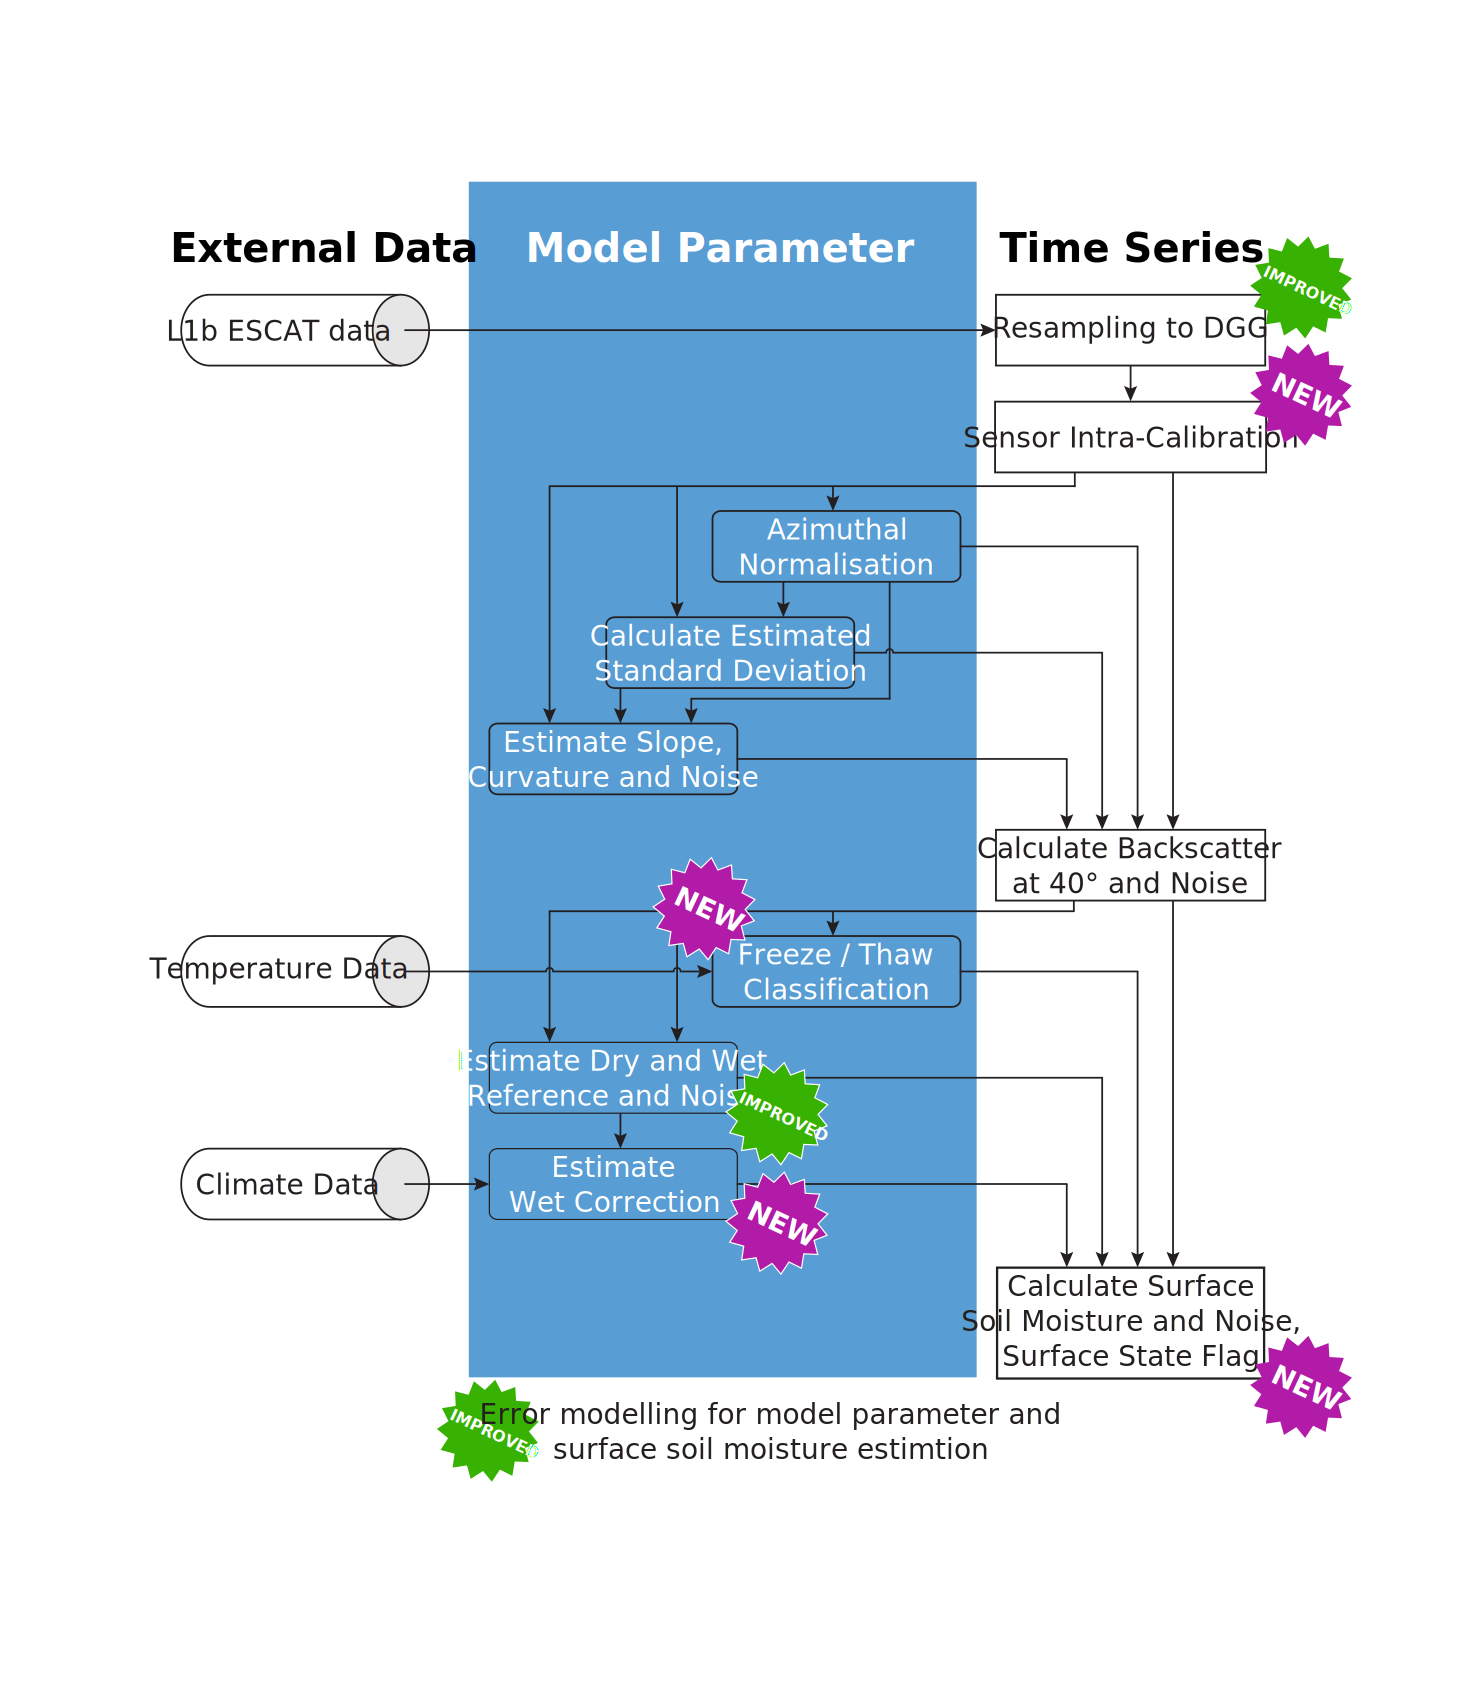
\includegraphics[width=0.7\blockwidth]{figures/WARP_processing_steps.pdf}
        \end{tikzfigure}
      \end{center}
    }


    \column{.5} 

    \block{Product Overview \phantom{Motivation}}{
      Soil Moisture products from ERS ESCAT are available in the Swath-Grid or Time-Series format.
      The Swath-Grid product is foreseen for NWP centers, to complement the operational disseminated ASCAT SM product from EUMETSAT, in support to NWP re-analysis and climate monitoring.
      For research and climate change studies a Time-Series product is accessible on a discrete global earth grid.
      Both soil moisture product families will be disseminated in NetCDF following the CF-conventions.

      \begin{center}
        \begin{tikzfigure}[Products.\label{figures:escat_products}] 
          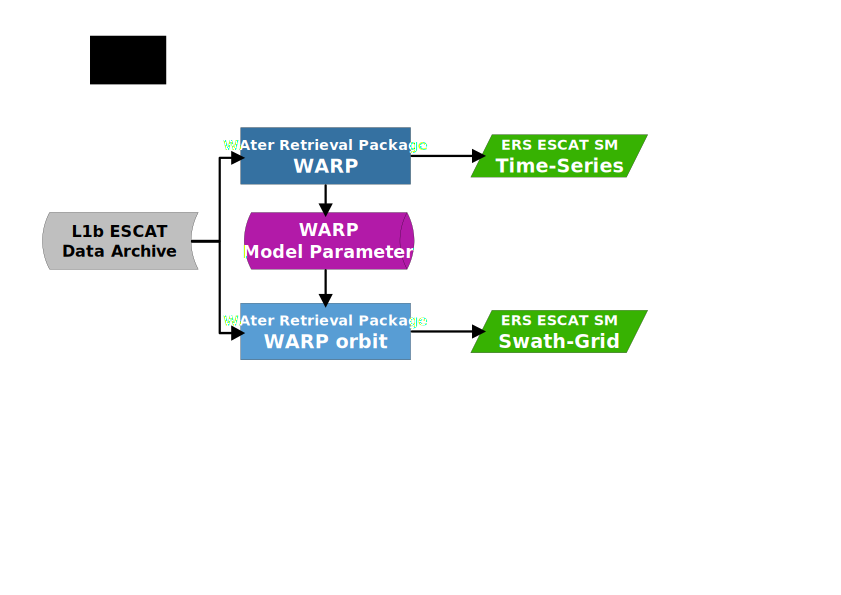
\includegraphics[width=0.6\blockwidth]{figures/WARP_WARPNRT.png}
        \end{tikzfigure}
      \end{center}
      
      \begin{center}
        \begin{tikzfigure}[ASPS Level 1 spatial resolution.\label{figures:spat_res}] 
          \includegraphics[width=0.8\blockwidth]{figures/ASPS_resolutions.png}
        \end{tikzfigure}
      \end{center}
 
    }

    \block{Validation Results}{
      A validation study has been carried out in order to analyze the performance of the newly computed ERS ESCAT Soil Moisture Products.
      The products have been validated against in-situ SM observations from the International Soil Moisture Network (ISMN) and land surface model predictions from ERA-Interim and GLDAS-NOAH.

      \begin{center}
        \begin{tikzfigure}[ISMN validation results utilizing Triple Collocation method to estimate the Signal to Noise Ratio (SNR)\label{figures:ismn_val}] 
          \includegraphics[width=0.45\columnwidth]{figures/TripleCol_SNR_R.png}
        \end{tikzfigure}
      \end{center}

      \begin{minipage}[t]{0.5\blockwidth}
        \begin{center}
          \begin{tikzfigure} 
            \includegraphics[width=0.49\blockwidth]{figures/WARP_SM_ERAINT_R_ALL_map.png}
          \end{tikzfigure}
        \end{center}
      \end{minipage}
      \begin{minipage}[t]{0.5\blockwidth}
        \begin{center}
          \begin{tikzfigure}
            \includegraphics[width=0.49\blockwidth]{figures/WARP_SM_GLDAS_R_ALL_map.png}
          \end{tikzfigure}
        \end{center}
      \end{minipage}
      \begin{minipage}[t]{\blockwidth}
        \begin{tikzfigure}[Land surface validation]
          \centering
        \end{tikzfigure}
      \end{minipage} 
    }
    
    \block{Access the Data}{ 
    }

  \end{columns}

\end{document}
